\documentclass[letterpaper,10pt]{article}
\usepackage[top=2cm, bottom=1.5cm, left=1cm, right=1cm]{geometry}
\usepackage{amsmath, amssymb, amsthm,graphicx, enumitem}
\usepackage{fancyhdr}
\pagestyle{fancy}

\lhead{\today}
\chead{MSCS 791 Progress Report 2}
\rhead{Justin Hood}

\newcommand{\Z}{\mathbb{Z}}
\newcommand{\Q}{\mathbb{Q}}
\newcommand{\R}{\mathbb{R}}
\newcommand{\C}{\mathbb{C}}
\newtheorem{lem}{Lemma}

\begin{document}
Over the last few weeks I have gotten a large amount accomplished, with no small amount of setbacks. In summary,
\begin{itemize}
\item I have built my discrete event modeler in C++
\item I have resolved several issues in the logic of the code that included issues with:
\begin{itemize}
\item Number of Workers not remaining constant
\item Worker job assignments not sticking
\item Script throughput time causing cascading issues throughout the code as Segfaults and memory access crashes.
\end{itemize}
\item Setup the R framework to analyze the results of my output data (Cleaning up my csv files and some plots- see below)
\item Setup the C++ framework for several potential optimizations. Not run yet, as I am waiting to see what you think of the results for my base case.
\end{itemize}
As of now, my current simulation parameters are,
\begin{itemize}
\item Number of Hours: 12
\item Number of Updates per Minute: 4 (Every 15 seconds)
\item Number of Pharmacists: 2
\item Number of Techs: 5 (4 Normal and 1 IV)
\item Number of Trials: 30
\end{itemize}
I chose the 30 trials as it is sufficient for CLT assumptions of normality, and I wanted to keep the number of trials limited, as increased numbers of trials rely too heavily on our assumed parameters for the sampling distribution, and does not provide particularly interesting results. Running my model with the above parameters, I obtain the following 95 \% intervals:
\begin{align*}
\text{Oral Incoming} &= [91.69264,\ 97.70736] && \text{Number of Orders}\\
\text{IV Incoming} &= [41.48018,\ 46.11982] && \text{Number of Orders}\\\\
\text{Entry Queue} &= [0.3995144,\ 0.5428235] && \text{Number of Orders}\\
\text{Entry Verification Queue} &= [7.356473,\ 11.06084] && \text{Number of Orders}\\
\text{Oral Fill Queue} &= [0.1261225,\ 0.1614932] && \text{Number of Orders}\\
\text{IV Fill Queue} &= [0.0566676,\ 0.08567036] && \text{Number of Orders}\\
\text{Fill Verification Queue} &= [3.918231,\ 6.045171] && \text{Number of Orders}\\
\text{Dispense Queue} &= [0.2207893,\ 0.2724746] && \text{Number of Orders}\\\\
\text{Oral Filled} &= [67.55312,\ 70.91354] && \text{Number of Orders}\\
\text{IV Filled} &= [30.55001,\ 34.78332] && \text{Number of Orders}\\\\
\text{Pharmacist Idle Time} &= [3.350241,\ 4.793278] && \text{Percent of Total Time}\\
\text{Technician Idle Time} &= [17.70447,\ 20.13233] && \text{Percent of Total Time}\\
\text{IV Technician Idle Time} &= [69.77078,\ 73.3357] && \text{Percent of Total Time}\\\\
\text{Oral Throughput Times} &= [104.115,\ 130.0625] && \text{Minutes}\\
\text{IV Throughput Times} &= [88.9775,\ 118.2537] && \text{Minutes}\\\\
\end{align*}
These are displayed graphically below,
\begin{center}
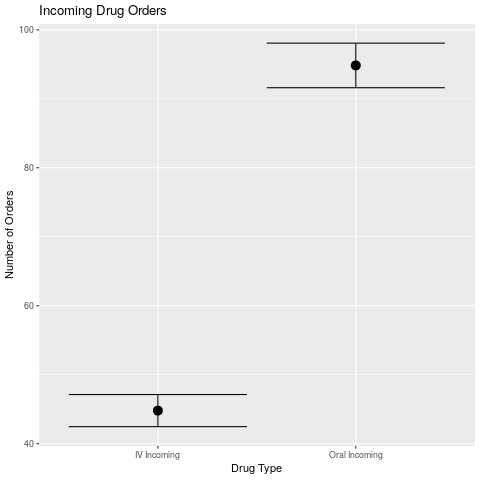
\includegraphics[scale=.5]{IncomingCIs.png}
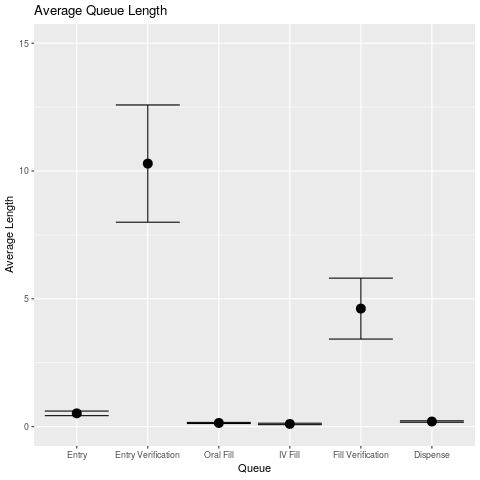
\includegraphics[scale=.5]{QueueCIs.png}\\
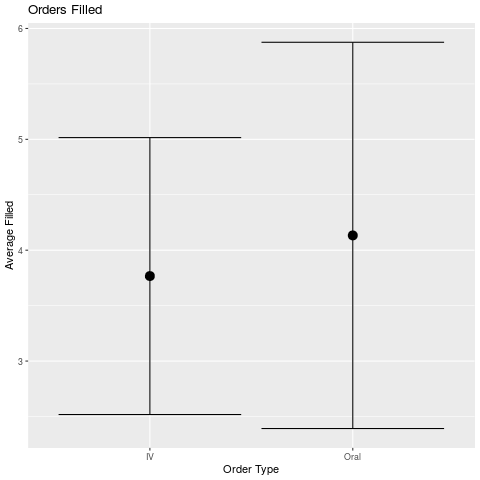
\includegraphics[scale=.5]{FilledCIs.png}
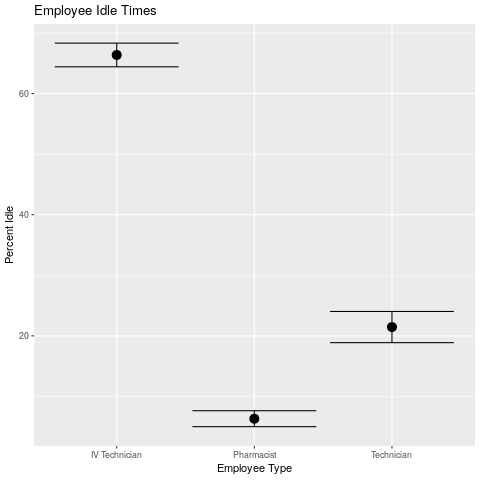
\includegraphics[scale=.5]{IdleCIs.png}\\
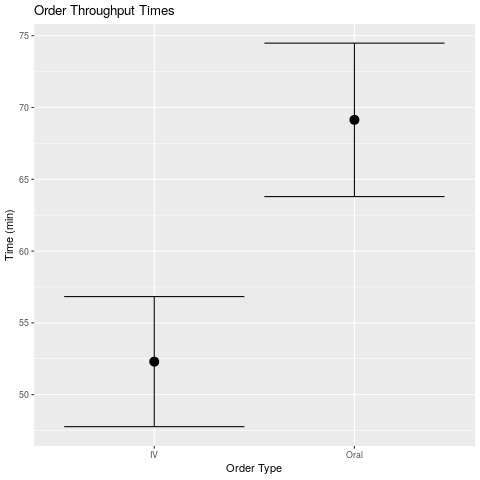
\includegraphics[scale=.5]{ThroughputCIs.png}
\end{center}
While it is clear from the numerical results, the graphs make it very clear that the main bunching points of the process flow are the verification steps. This is to be expected, as in our base model the pharmacists do not prioritize these orders in the workflow, instead, they only account for 40\% of the potential tasks they perform.\\\\
I am slightly behind my proposed timeline, but this is mainly due to the issues that I hope I have resolved. As I stated before, running the confidence analysis on my theorized optimizations should take under 5 minutes, as it is merely a matter of executing the code that I have already written, which I will do once I have the OK from you on my base case.\\\\
I have some questions on how I might be able to quantify improving the process, but I will save these until I reach that point in the process.\\\\
Assuming that my analysis for the base case looks good, I will run my optimizations and discuss with you what improvements I think are best, and then begin the rough draft of my project.\\\\\\
Note: I am sorry for the ``Radio Silence" from your last email. I updated my phone, and it logged me out of my school email account, so I did not see your email last week.
\end{document}
